\documentclass[twocolumn,9pt,a4paper]{jsarticle}
%
\usepackage{amsmath,amssymb}
\usepackage{bm}
\usepackage{epsbox}
\usepackage[dvipdfmx]{graphicx}
\usepackage{verbatim}
\usepackage{wrapfig}
\usepackage{ascmac}
\usepackage{makeidx}
\usepackage[dvipdfmx]{graphicx}

\usepackage{listings, jlisting}
\usepackage{color}
 
\lstset{
    language=Python,%プログラミング言語によって変える。
    numbers = left,
    numberstyle = {\tiny \emph},
    numbersep = 10pt,
    breaklines = true,
    breakindent = 40pt,
    frame = tlRB,
    frameround = ffft,
    framesep = 3pt,
    rulesep = 1pt,
    rulecolor = {\color{black}},
    rulesepcolor = {\color{black}},
    flexiblecolumns = true,
    keepspaces = false,
    basicstyle = \scriptsize,
    identifierstyle = \itshape\scriptsize,
    commentstyle = \fontfamily{ptm}\selectfont\scriptsize,
    stringstyle = \scshape\scriptsize,
    tabsize = 4, 
 }

%
\setlength{\textwidth}{\fullwidth}
%\setlength{\textheight}{40\baselineskip}
\addtolength{\textheight}{\topskip}
\setlength{\voffset}{-0.2in}
\setlength{\topmargin}{0pt}
%\setlength{\headheight}{0pt}
%\setlength{\headsep}{0pt}
%
\newcommand{\divergence}{\mathrm{div}\,}  %ダイバージェンス
\newcommand{\grad}{\mathrm{grad}\,}  %グラディエント
\newcommand{\rot}{\mathrm{rot}\,}  %ローテーション
%
\title{Scratchプログラムの可視化による類似度推定}
\author{G13908 岩科智彩 G13924 森下汐美}
\date{平成29年1月31日}
\begin{document}
\maketitle
%
%
\section{はじめに}
近年プログラミング教育が推進され、日本でも小学校での導入が検討されている。子供のプログラミング教育の方法として近年よく利用されているのが米国マサチューセッツ工科大学のメディアラボが開発したScratchである。ScratchとはGUI環境を提供し、ブロックを組み合わせることでプログラムを作る。初心者にとっては使いやすい設計となっているため米国では利用者が増えている。また利用者同士ではプログラムを公開し共有するためのサイトも提供している。そこで実際にサイトで公表されているScratchプログラムを利用して、教育を支援するツールを目指すことにした。Scratchではあるプログラムが引用された場合、その関係をリミックスツリーという図で表している。これでは引用関係は分かるが実際に引用されたもの同士の類似度は表されていないため、一箇所の変更を加えたもの、多数の変更を加えたものはリミックスツリー上では引用元のプロジェクトから同距離で表されている。本研究ではリミックスツリー上では表されていない類似性の数値化を行い、より分かりやすく表示させることを目指した。

\section{Scratchの現状}
Scratchプロジェクトではあるプログラムが引用された場合、その関係をリミックスツリーという図で表している。この図では引用関係は分かるものの、実際に引用されたもの同士の類似度は表されていないため、一箇所の変更を加えたもの、多数の変更を加えたものはリミックスツリー上では引用元のプロジェクトから同距離で表されているのが現状である。この距離が数値化され、分かりやすく表されれば、例えば生徒の課題が提出された際にサンプルプログラムとの類似性で評価が分かりやすくできるのではないかと考える。

\section{提案する手法}
本研究では元プロジェクトと各プロジェクトをすべてのブロックが記録された1つの辞書型データを使用し、類似度推定を行う。類似度尺度はcos類似度を用いる(\cite{cos})。cos類似度とはベクトル空間モデルにおいて、文書同士を比較する際に用いられる類似度計算方法である。
\\
 収集できるScratchプロジェクトのデータはjson形式(\cite{json_py})であるため、Python環境のもとjsonモジュールをインポートすることでファイルを読み込む。Scratchでは数多くのブロックが用意されており、どのブロックを使用するかによって、まったく異なるプログラムを作成することができるため、本研究ではブロックの種類ごとの個数を集計をした後、ソートしたものをベクターに直すことで類似度計算を行う。また、使用されているブロック数とスプライト(オブジェクト)数も類似度を推定する際の要素として、使用する。
\\
\\【cos類似度】
\begin{equation}
\cos(A,B) = \frac{\vec{A} \ast\vec{B}} {|\vec{A}||\vec{B}|}  = \frac{\vec{A}}{|\vec{B}|}\ast\frac{\vec{A}}{|\vec{B}|} = \frac{\sqrt {\sum_{i=1}^{|V|}}}{\sqrt{\sum_{i=1}^{|V|}A_i^2\ast\sum_{i=1}^{|V|}B_i^2}}
\end{equation}


\section{実験方法}
本研究では2万弱の引用がされている"Pong Starter"(卓球ゲーム)のプロジェクト大規模なリミックスツリー(\cite{pongret})と200弱の引用がされている"Maze Game"(迷路ゲーム)の小規模なリミックスツリー(\cite{mazeret})を利用し、元プロジェクトと各プロジェクトを比較をした。使用されているブロック・スプライトを数え上げ、類似度を表すcos類似度を数値化し、これらのデータを使用してグラフ化する。元のプログラムから引用されたものを1段目、以後1段目のプロジェクトから引用されたものを2段目、2段目から引用されたものを3段目とし、各段ごとにグラフを作成する。

\section{実験結果}
出力されたデータを組み合わせてさまざまな可視化を行った。散布図では縦軸にcos類似度の値、横軸に出力されたブロック数(スプライト数)を元のプログラムの数値で割った値をとり、"Pong Starter"の場合はさらに対数値をとる。グラフ上では(1,1)が最も類似しているプロジェクトであるため、この点から同距離のものを似ているものから順に青、赤、緑、紫、水色と区別してプロットをする。カラーマップでは各要素の個数を集計し、頻度の高いものから色別でプロットした。
\\
\subsection{Pong Starter}
\subsubsection{ブロック数とcos類似度の散布図}
\begin{figure}[h]
 \begin{tabular}{cc}
 	\begin{minipage}[t]{0.45\hsize}
	 \centering
	 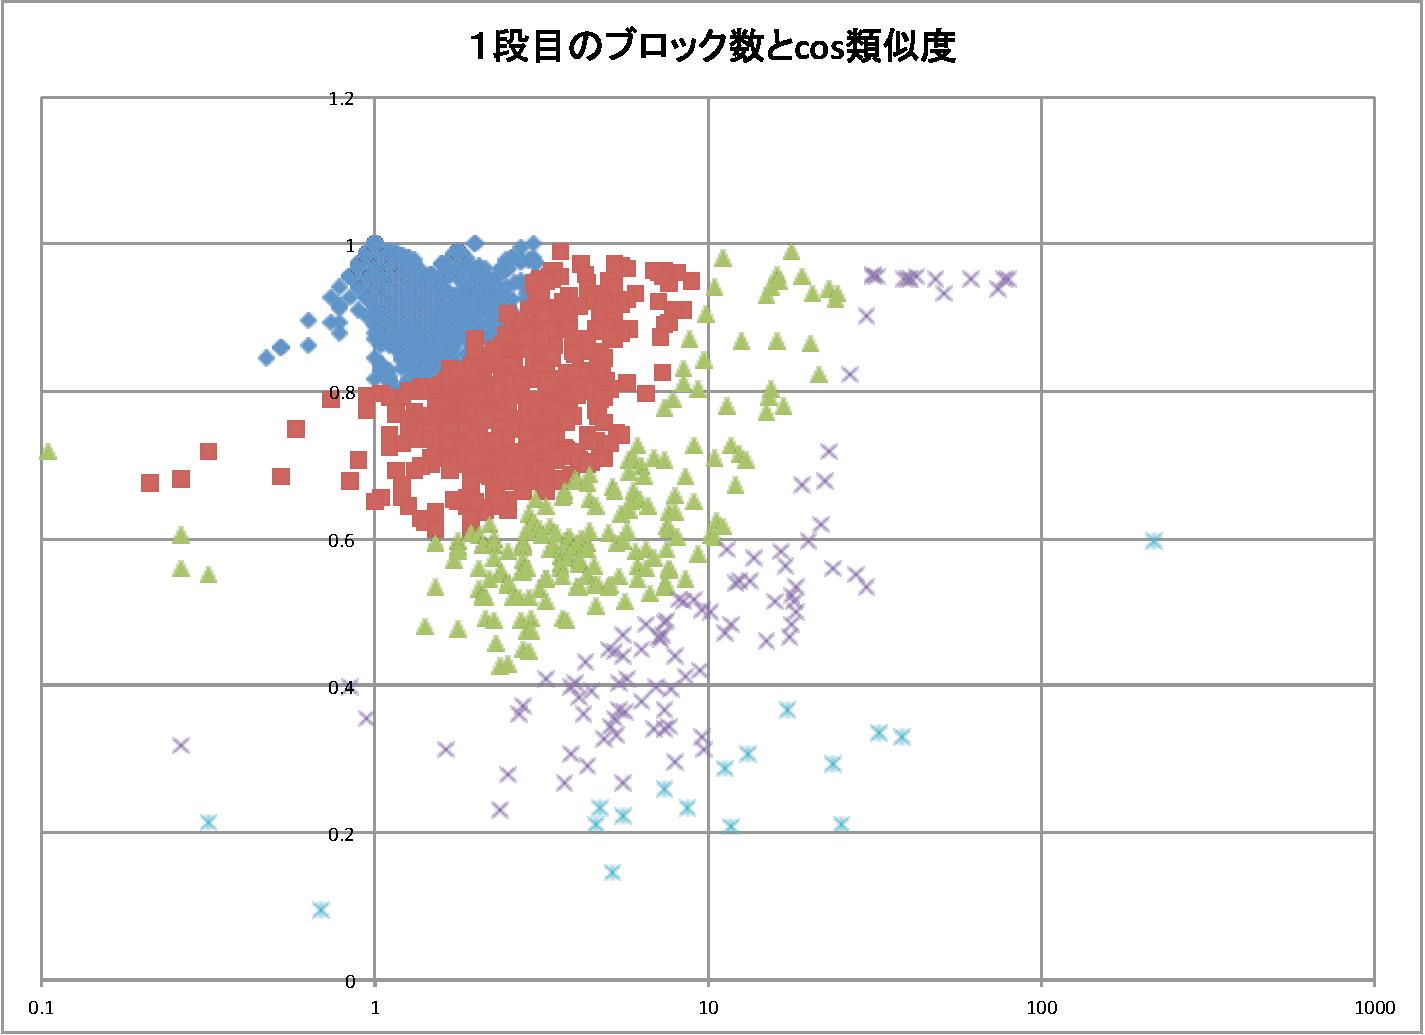
\includegraphics[keepaspectratio, scale = 0.15]{graph_1_block.pdf}
	 \caption{1段目のグラフ}
	 \label{first_block}
	\end{minipage}
        \begin{minipage}[t]{0.45\hsize}
	 \centering
	 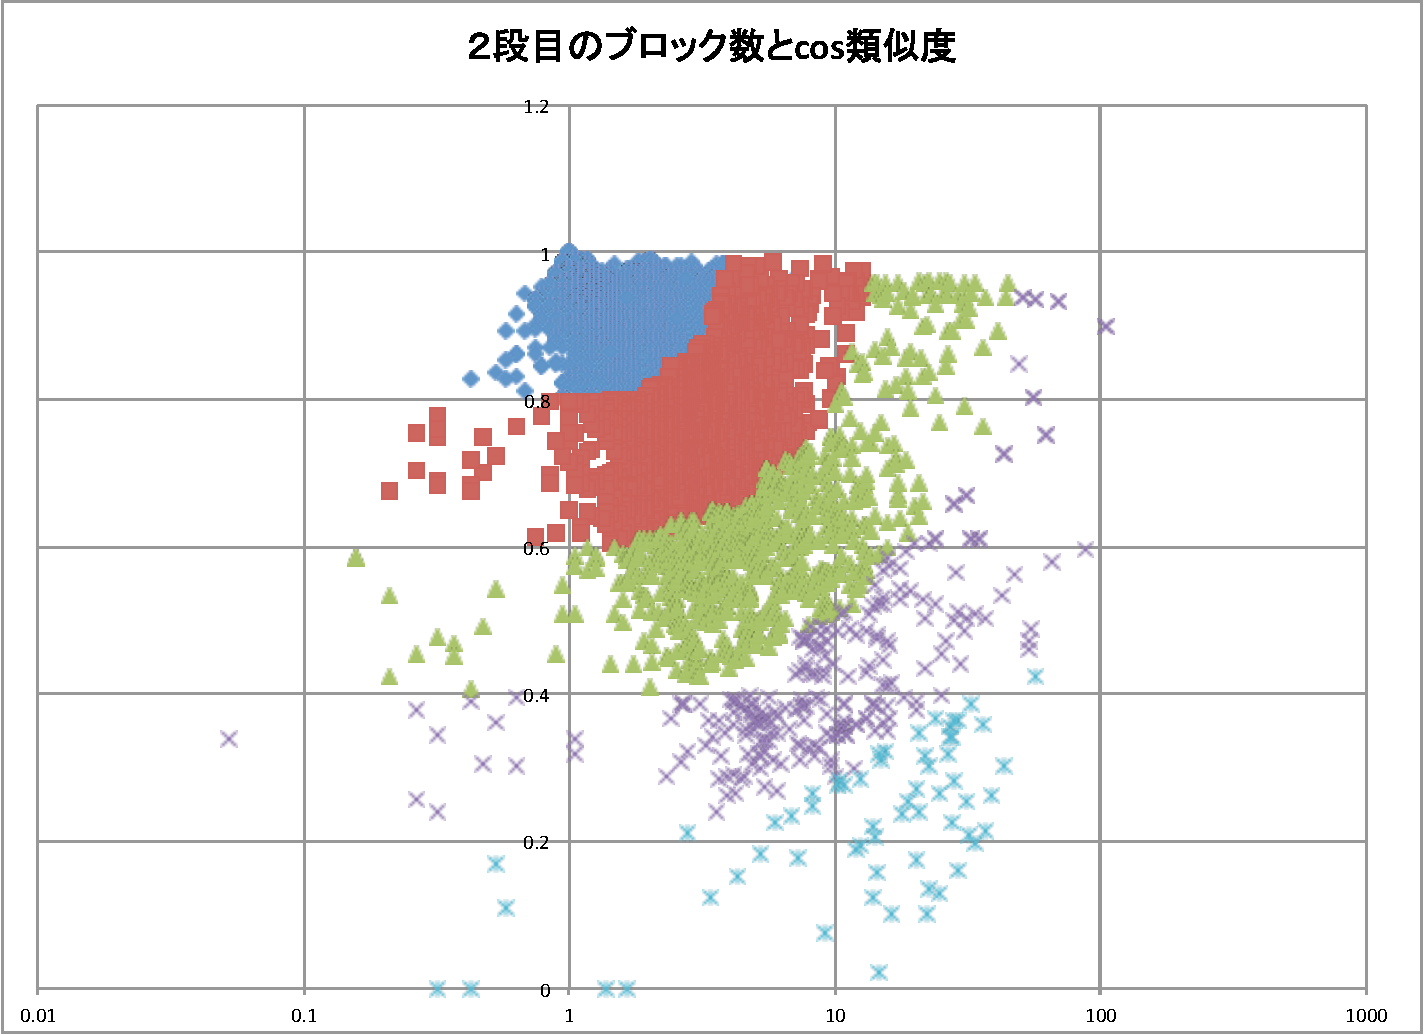
\includegraphics[keepaspectratio, scale = 0.15]{graph_2_block.pdf}
	 \caption{2段目のグラフ}
	 \label{second_block}
	\end{minipage}
 \end{tabular}
  \begin{tabular}{cc}
 	\begin{minipage}[t]{0.45\hsize}
	 \centering
	 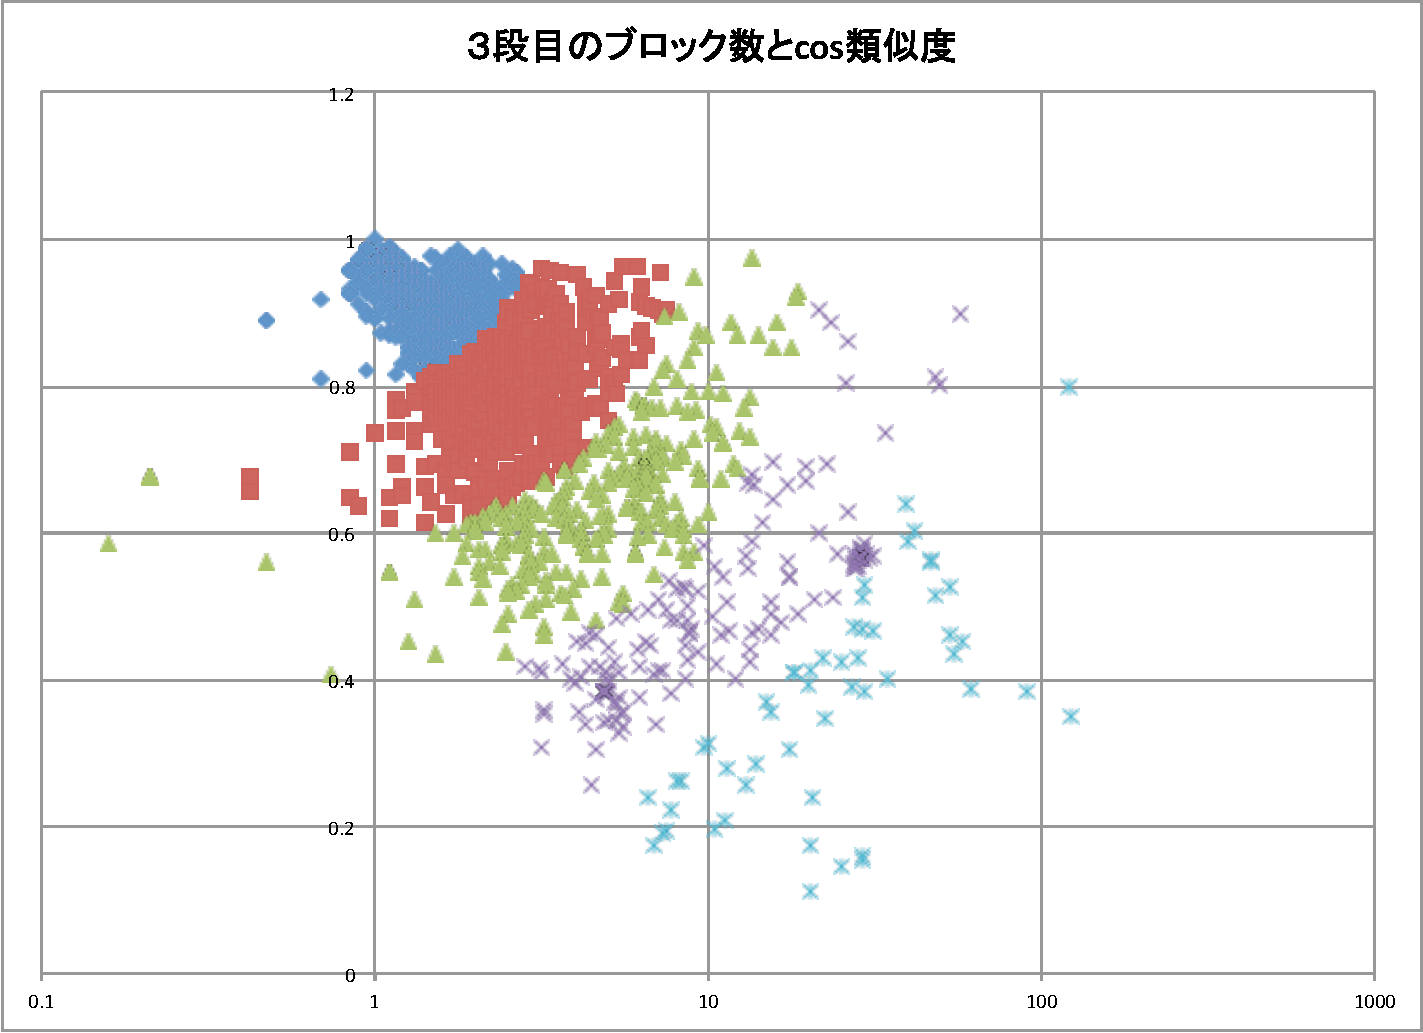
\includegraphics[keepaspectratio, scale = 0.15]{graph_3_block.pdf}
	 \caption{3段目のグラフ}
	 \label{third_block}
	\end{minipage}
        \begin{minipage}[t]{0.45\hsize}
	 \centering
	 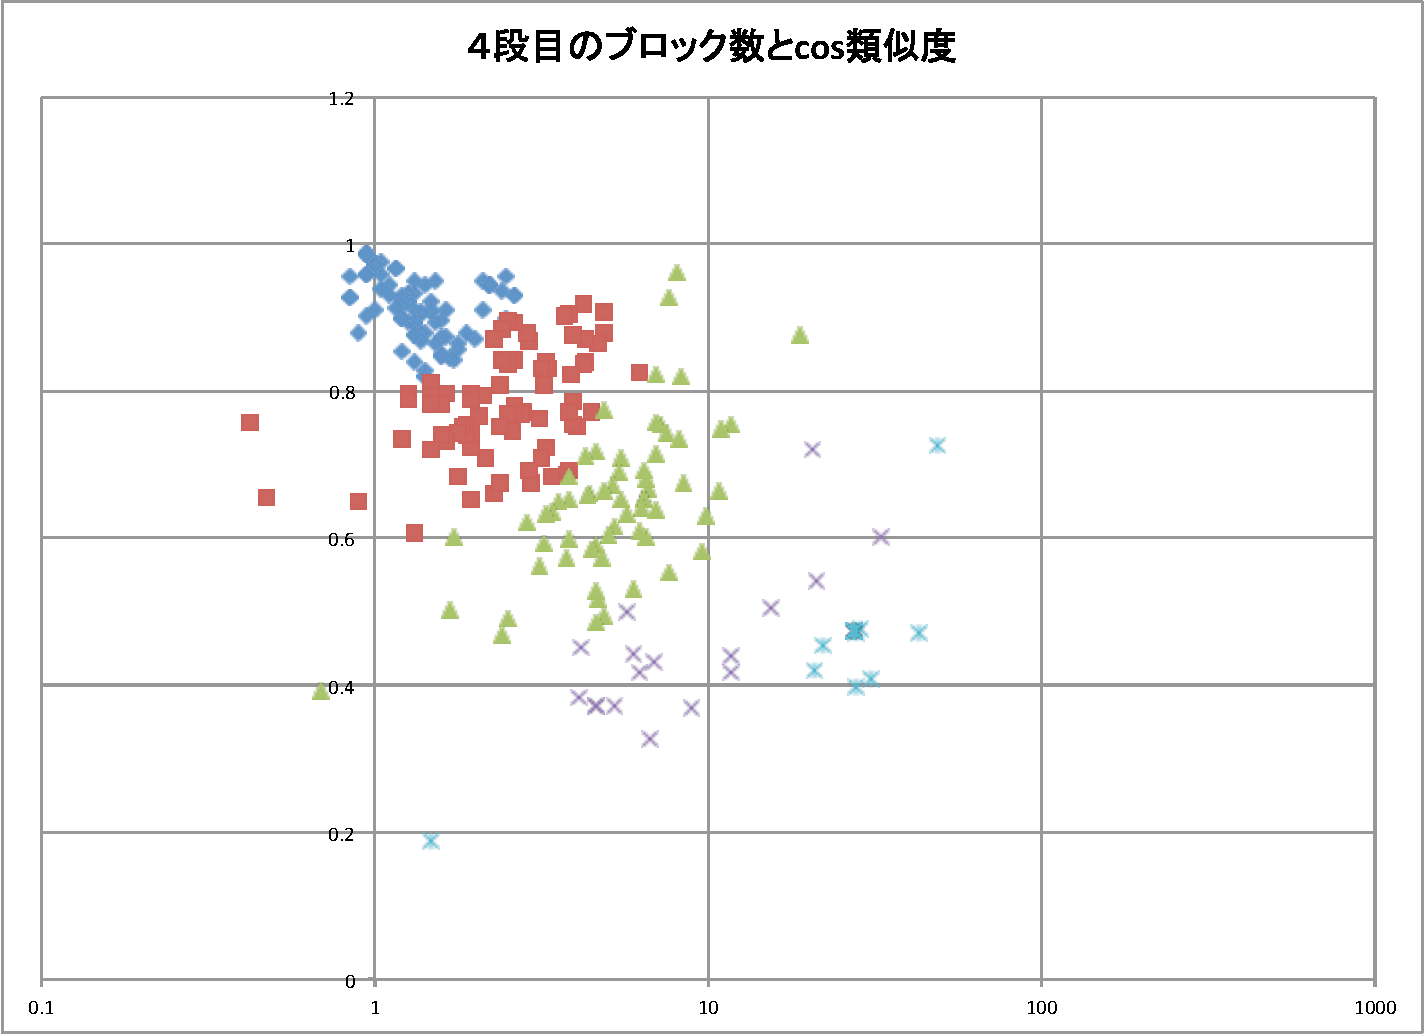
\includegraphics[keepaspectratio, scale = 0.15]{graph_4_block.pdf}
	 \caption{4段目のグラフ}
	 \label{fourth_block}
	\end{minipage}
 \end{tabular}
 \end{figure}

\subsubsection{スプライト数とcos類似度の散布図}
\begin{figure}[ht]
 \begin{tabular}{cc}
 	\begin{minipage}[t]{0.45\hsize}
	 \centering
	 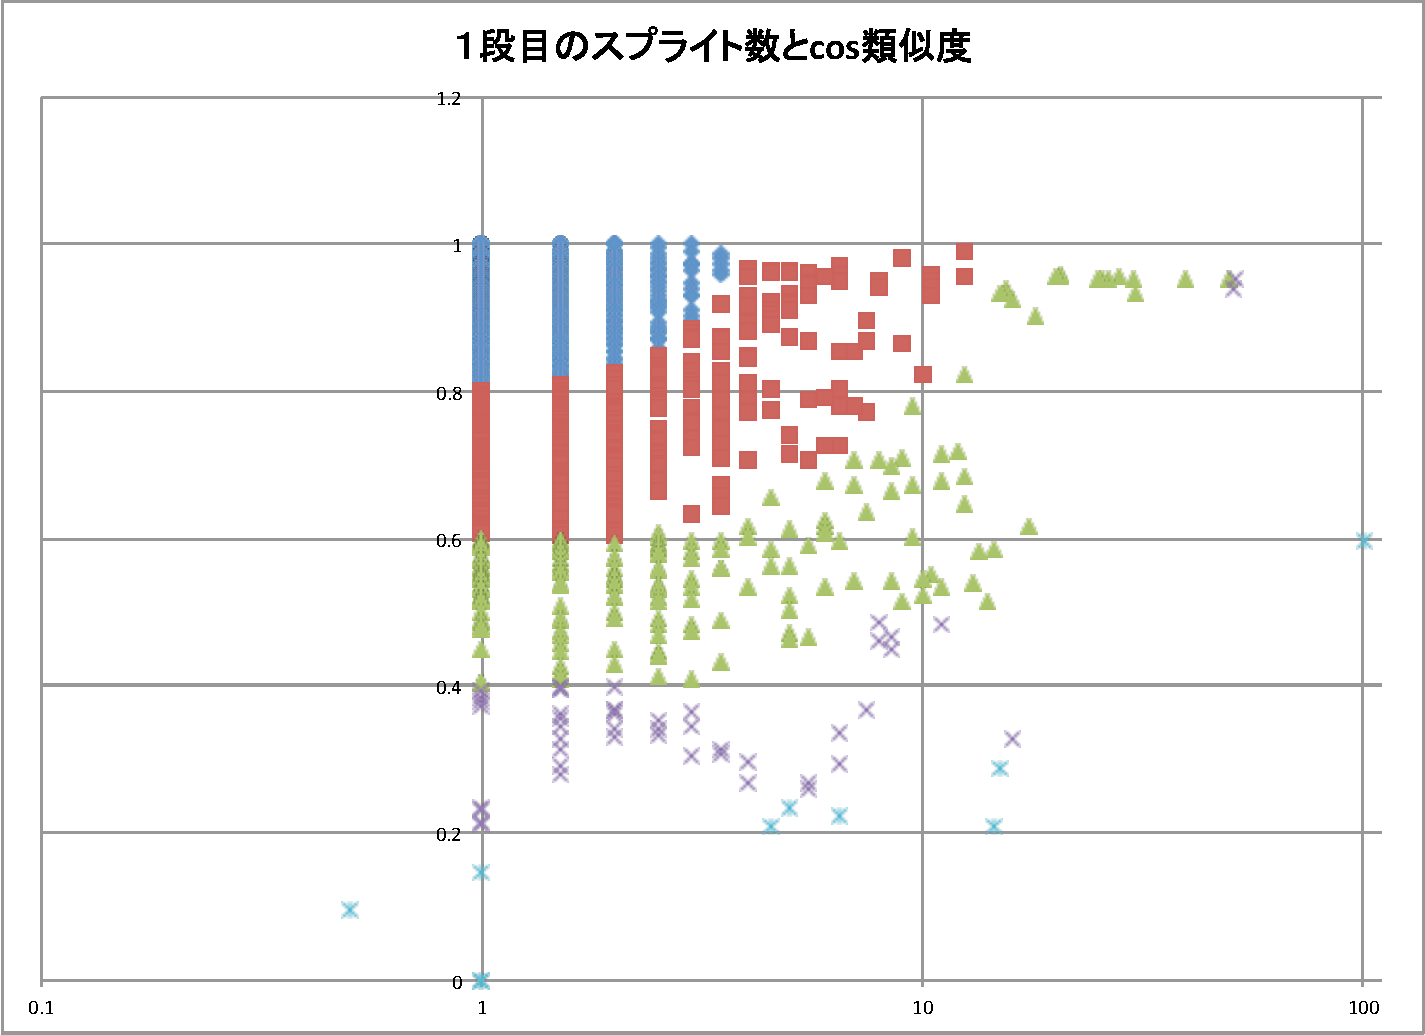
\includegraphics[keepaspectratio, scale = 0.15]{graph_1_splite.pdf}
	 \caption{1段目のグラフ}
	 \label{first_splite}
	\end{minipage}
        \begin{minipage}[t]{0.45\hsize}
	 \centering
	 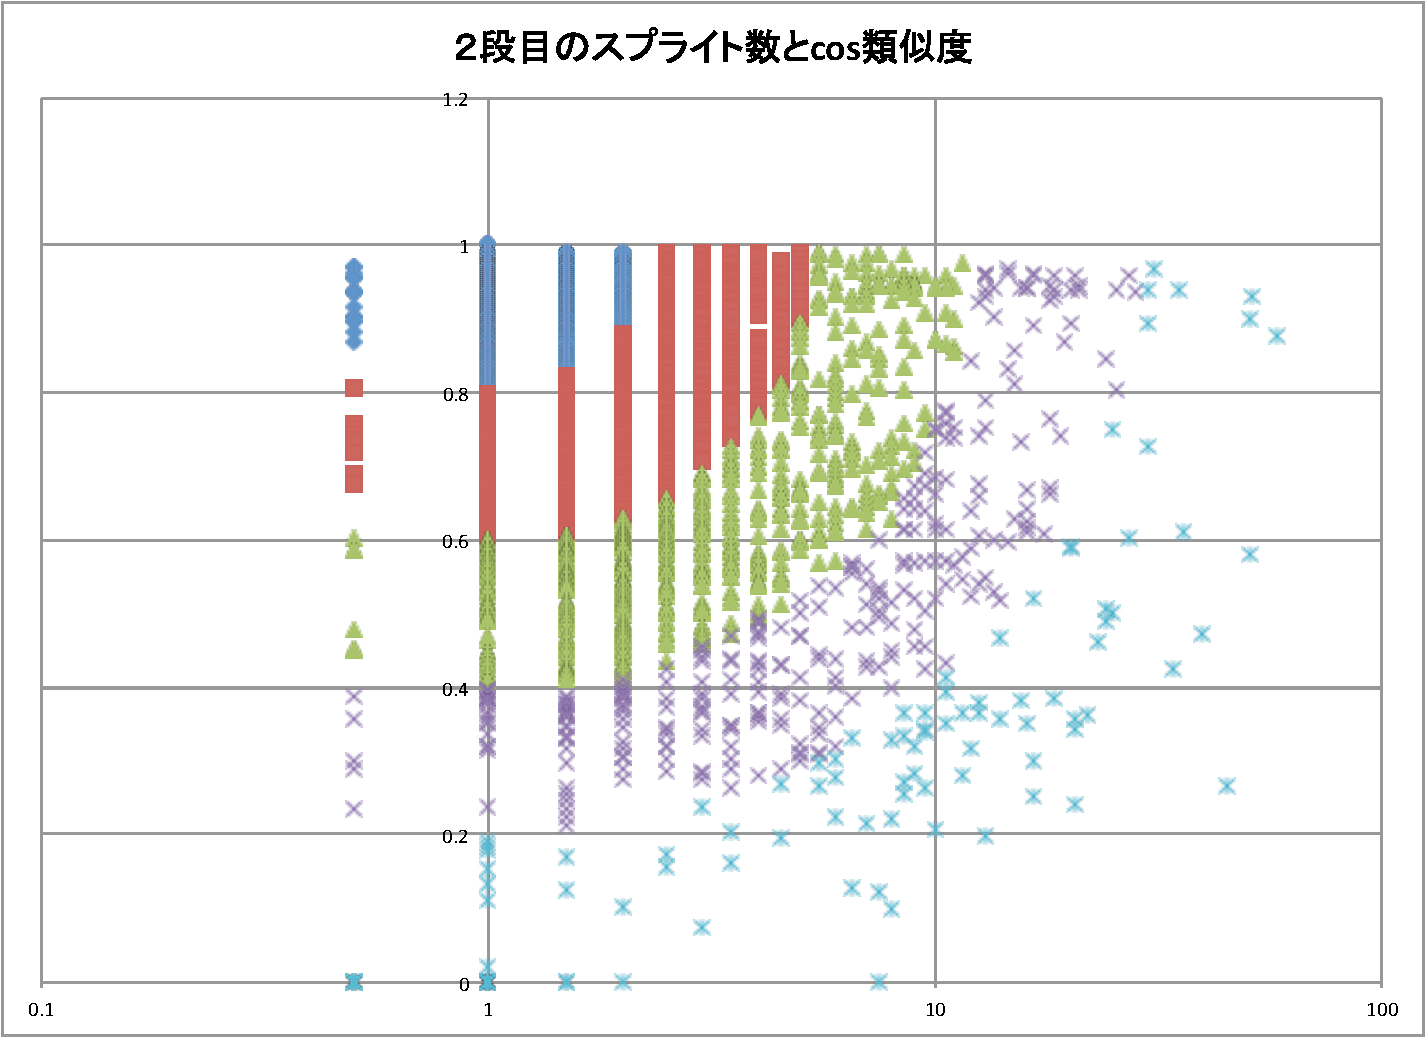
\includegraphics[keepaspectratio, scale = 0.15]{graph_2_splite.pdf}
	 \caption{2段目のグラフ}
	 \label{second_splite}
	\end{minipage}
 \end{tabular}
  \begin{tabular}{cc}
 	\begin{minipage}[t]{0.45\hsize}
	 \centering
	 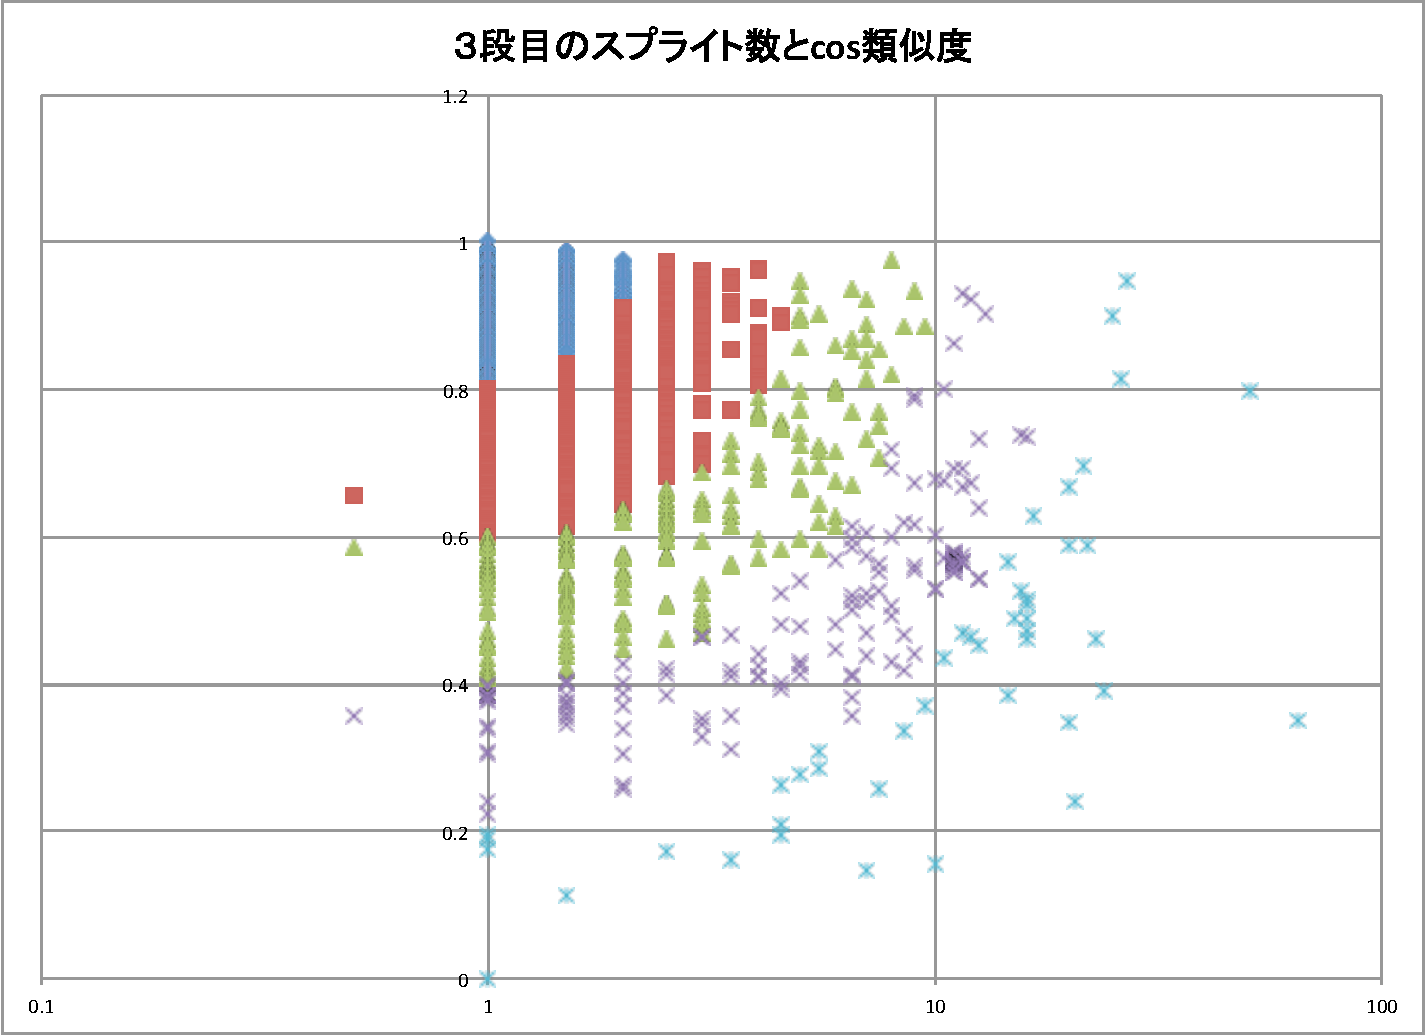
\includegraphics[keepaspectratio, scale = 0.15]{graph_3_splite.pdf}
	 \caption{3段目のグラフ}
	 \label{third_splite}
	\end{minipage}
        \begin{minipage}[t]{0.45\hsize}
	 \centering
	 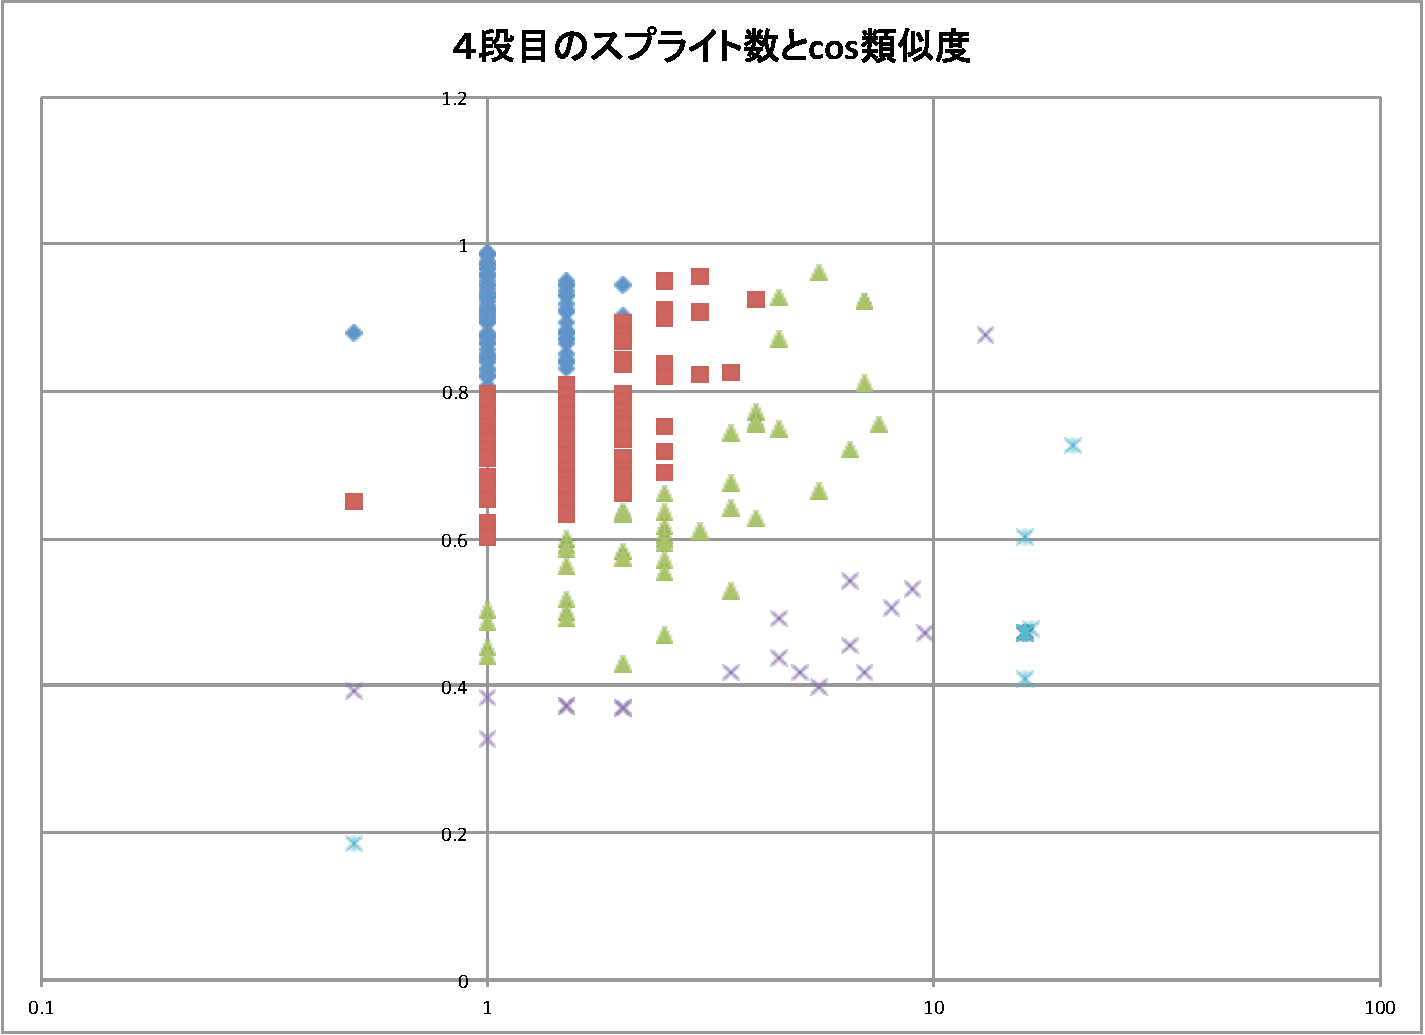
\includegraphics[keepaspectratio, scale = 0.15]{graph_4_splite.pdf}
	 \caption{4段目のグラフ}
	 \label{fourth_splite}
	\end{minipage}
 \end{tabular}
 \end{figure}

\newpage
 \subsubsection{ブロック数とcos類似度のカラーマップ}
\begin{figure}[ht]
 \begin{tabular}{cc}
 	\begin{minipage}[t]{0.45\hsize}
	 \centering
	 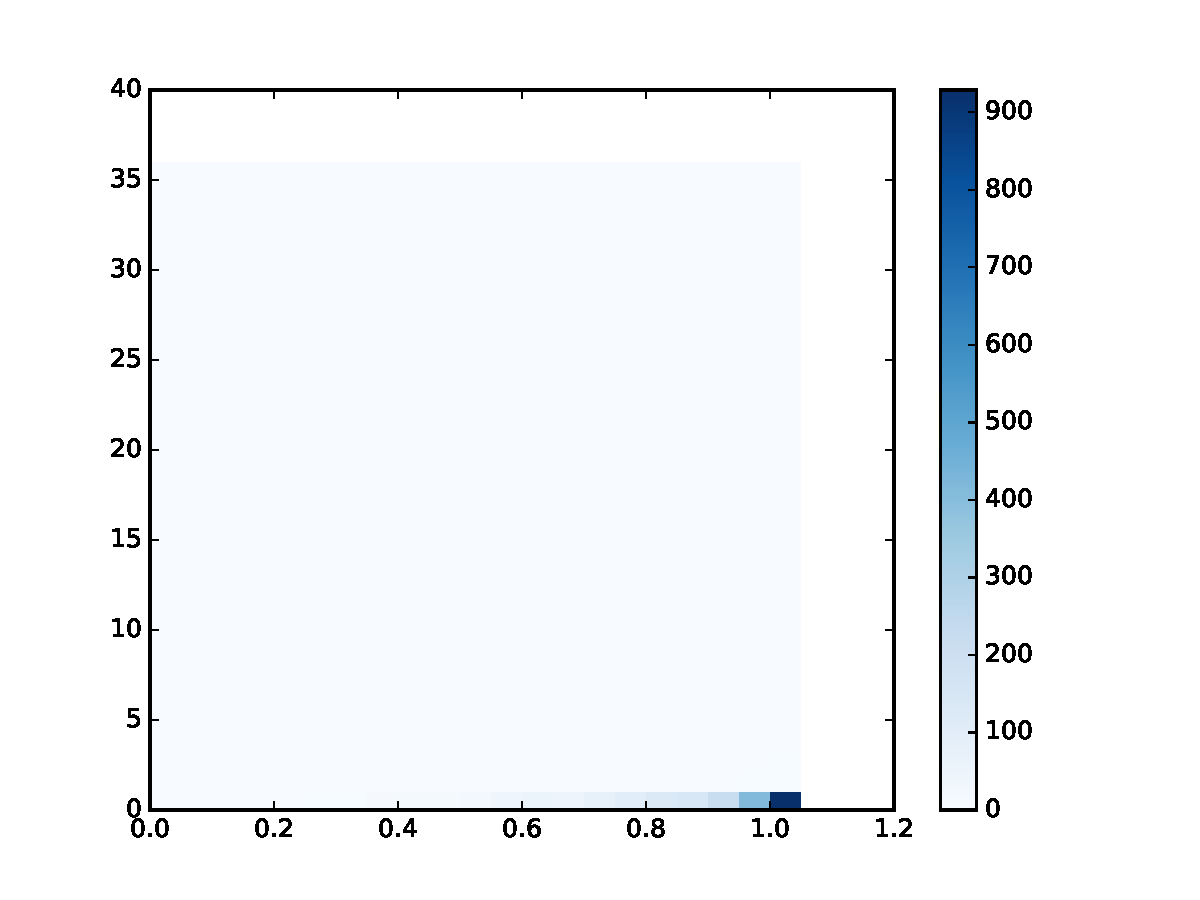
\includegraphics[keepaspectratio, scale = 0.2]{colormap_block_1.pdf}
	 \caption{1段目のグラフ}
	 \label{first_splite}
	\end{minipage}
        \begin{minipage}[t]{0.45\hsize}
	 \centering
	 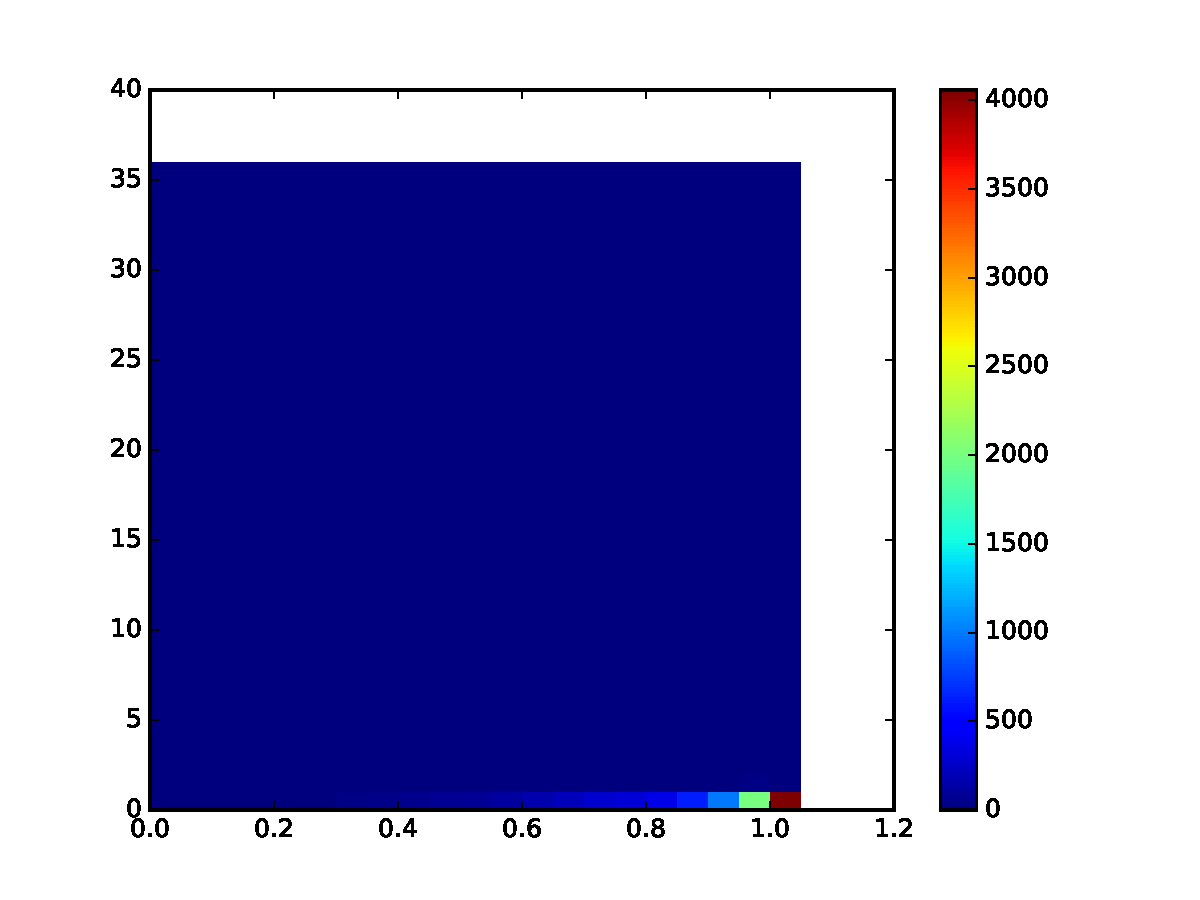
\includegraphics[keepaspectratio, scale = 0.2]{colormap_block_2.pdf}
	 \caption{2段目のグラフ}
	 \label{second_splite}
	\end{minipage}
 \end{tabular}
  \begin{tabular}{cc}
 	\begin{minipage}[t]{0.45\hsize}
	 \centering
	 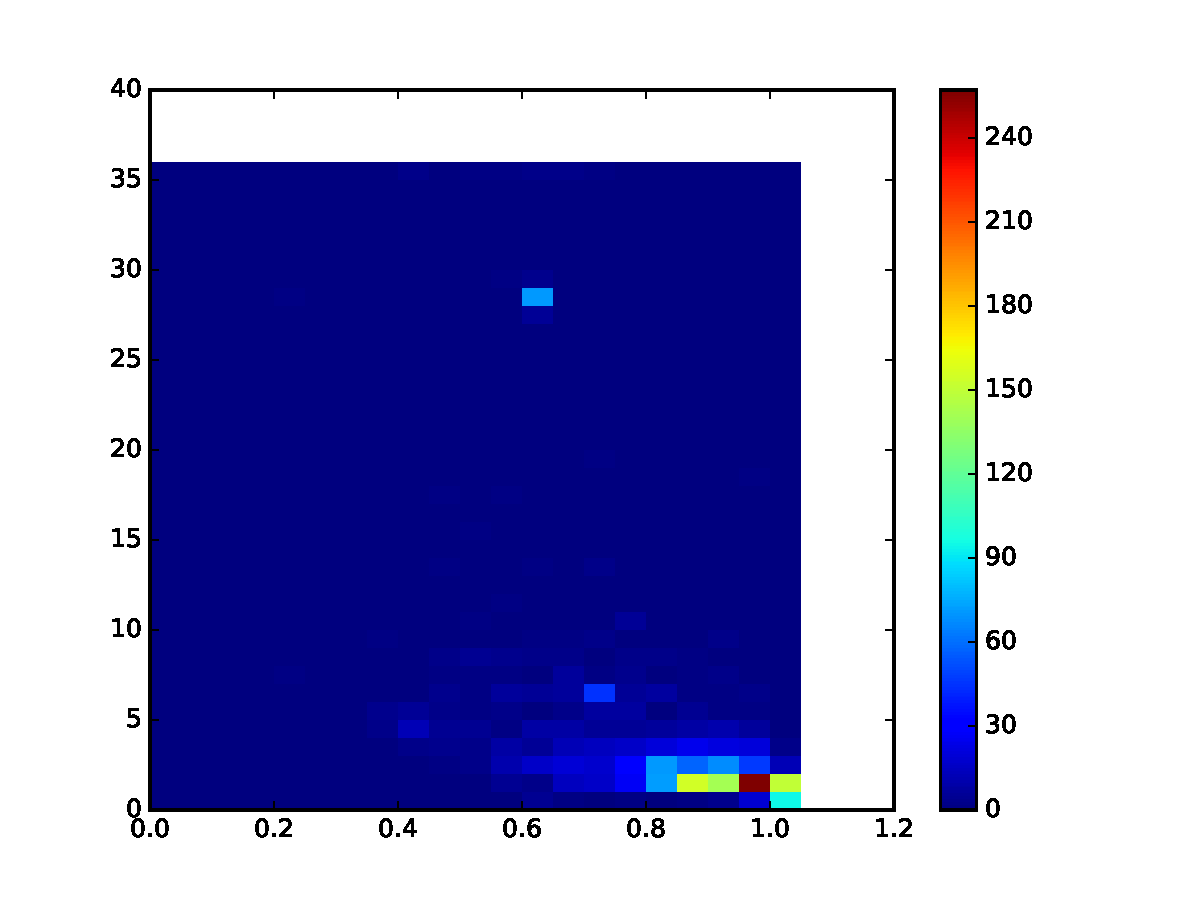
\includegraphics[keepaspectratio, scale = 0.2]{colormap_block_3.pdf}
	 \caption{3段目のグラフ}
	 \label{third_splite}
	\end{minipage}
        \begin{minipage}[t]{0.45\hsize}
	 \centering
	 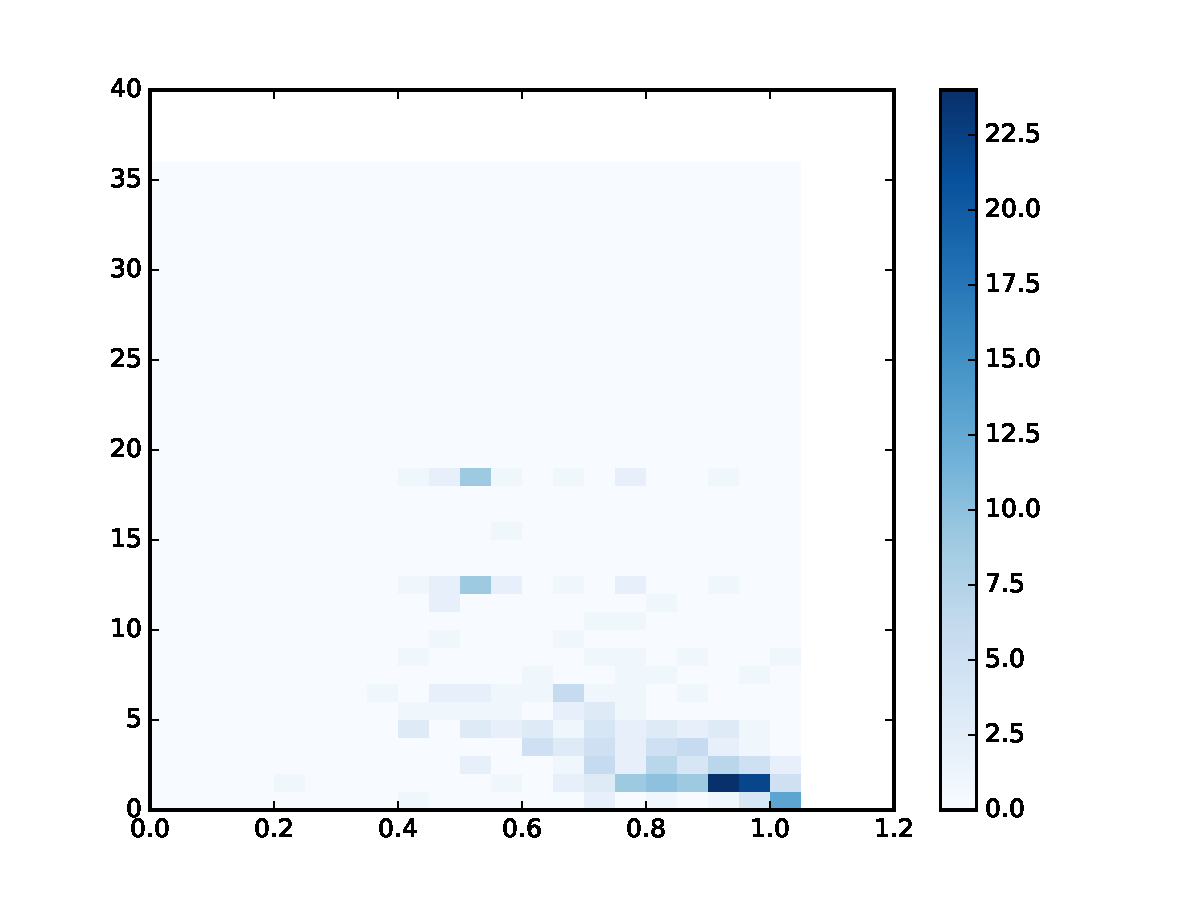
\includegraphics[keepaspectratio, scale = 0.2]{colormap_block_4.pdf}
	 \caption{4段目のグラフ}
	 \label{fourth_splite}
	\end{minipage}
 \end{tabular}
 \end{figure}
 
\subsubsection{スプライト数とcos類似度のカラーマップ}
\begin{figure}[h]
 \begin{tabular}{cc}
 	\begin{minipage}[t]{0.45\hsize}
	 \centering
	 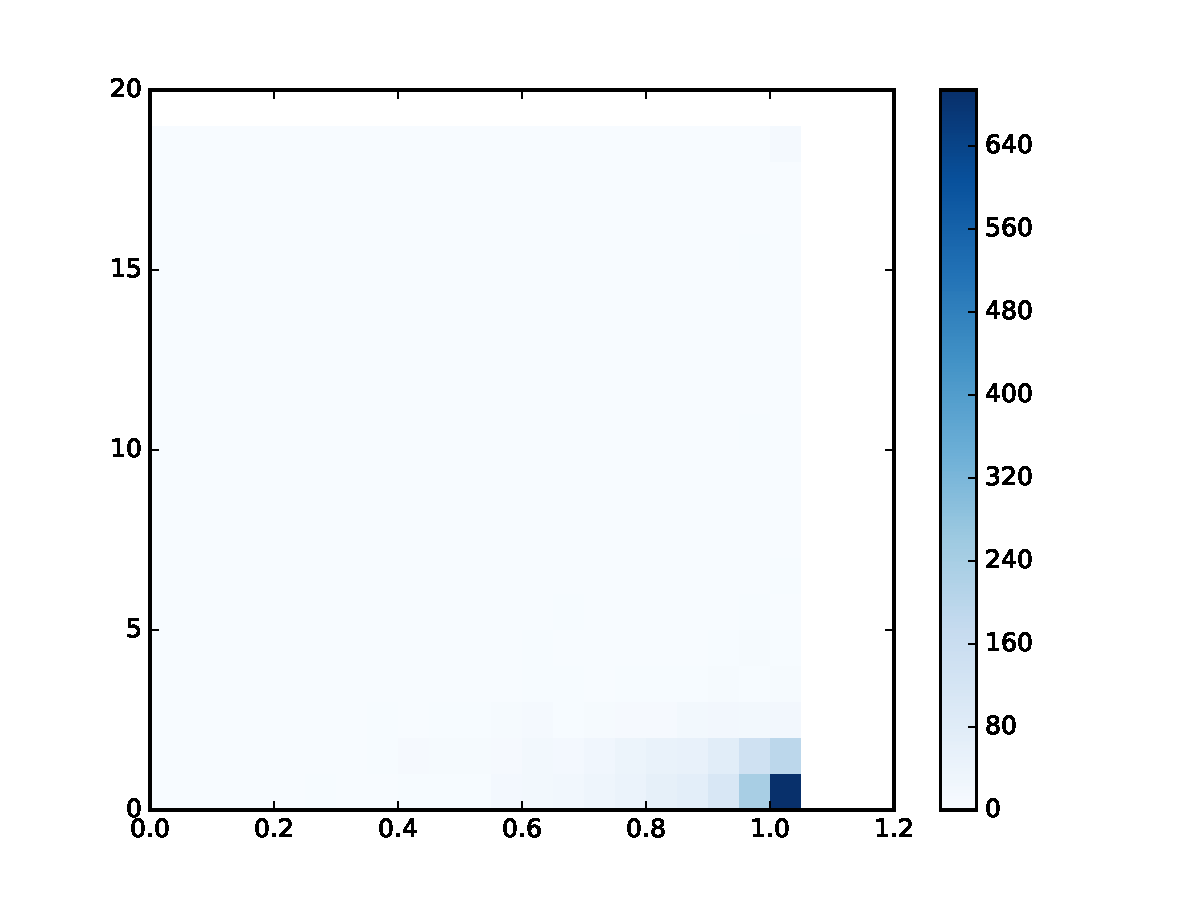
\includegraphics[keepaspectratio, scale = 0.2]{colormap_splite_1.pdf}
	 \caption{1段目のグラフ}
	 \label{first_splite}
	\end{minipage}
        \begin{minipage}[t]{0.45\hsize}
	 \centering
	 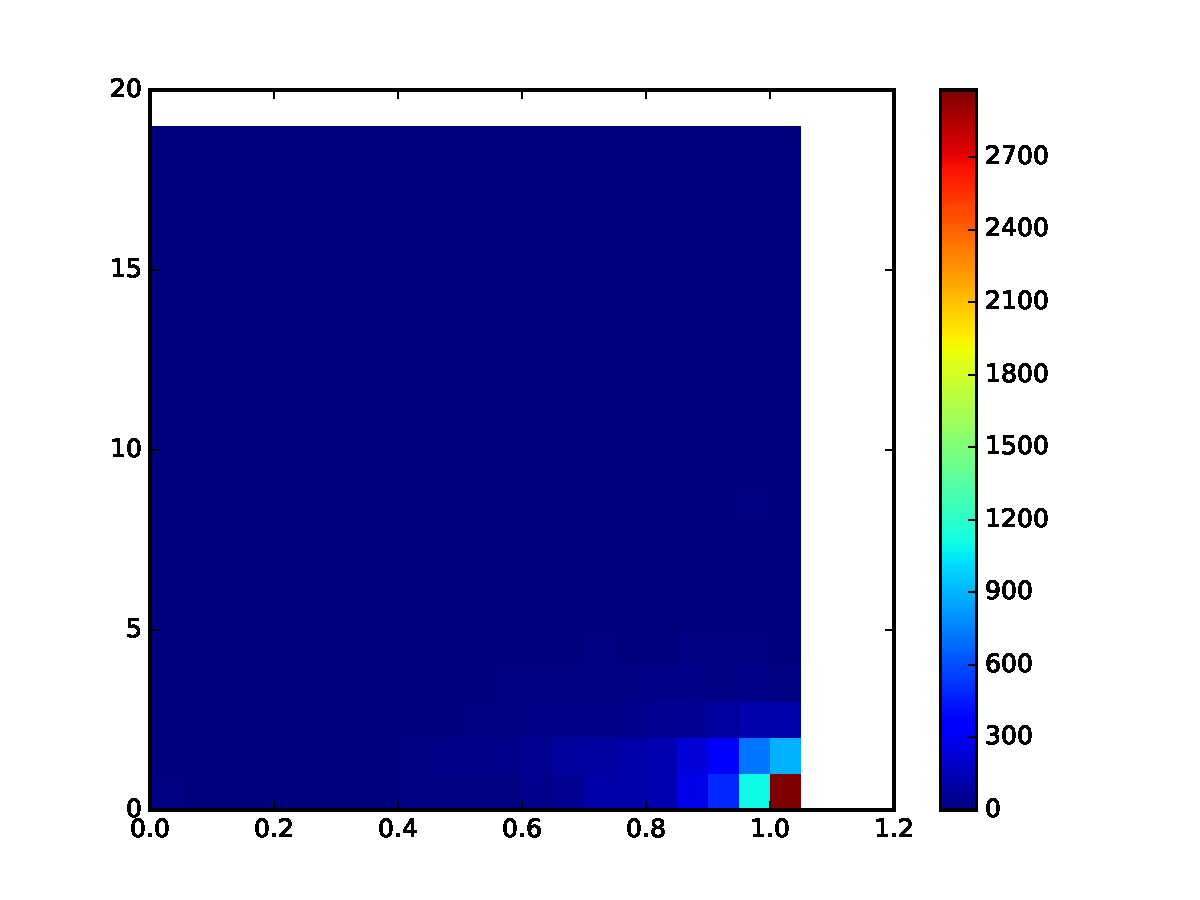
\includegraphics[keepaspectratio, scale = 0.2]{colormap_splite_2.pdf}
	 \caption{2段目のグラフ}
	 \label{second_splite}
	\end{minipage}
 \end{tabular}
  \begin{tabular}{cc}
 	\begin{minipage}[t]{0.45\hsize}
	 \centering
	 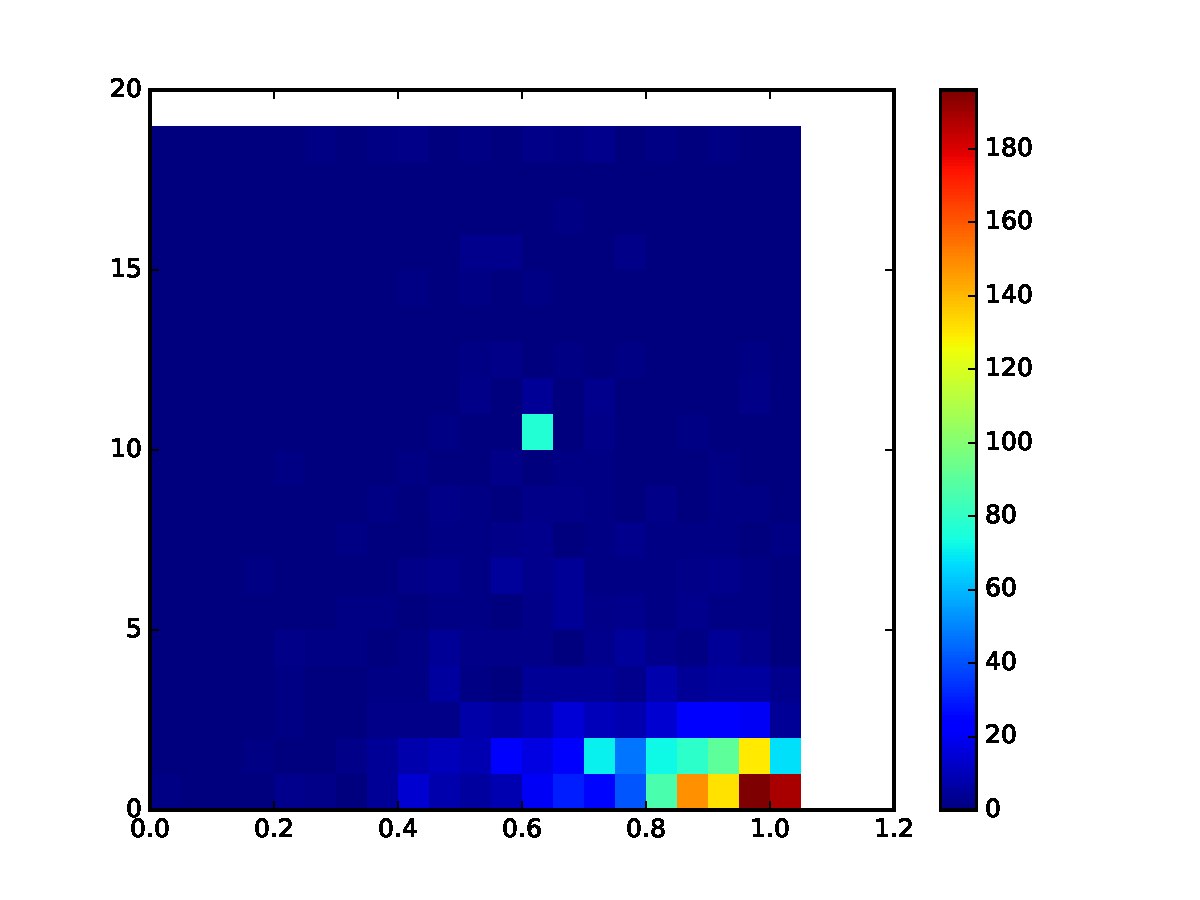
\includegraphics[keepaspectratio, scale = 0.2]{colormap_splite_3.pdf}
	 \caption{3段目のグラフ}
	 \label{third_splite}
	\end{minipage}
        \begin{minipage}[t]{0.45\hsize}
	 \centering
	 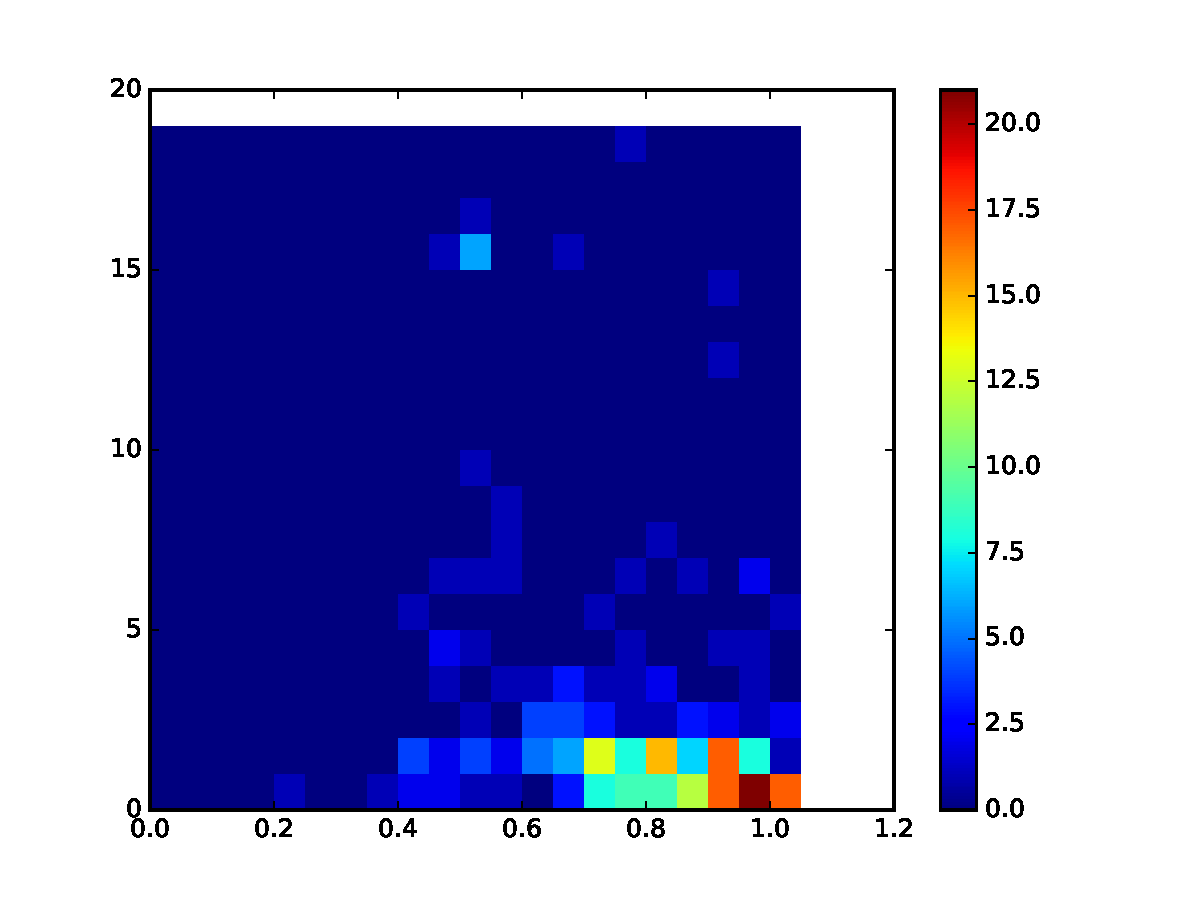
\includegraphics[keepaspectratio, scale = 0.2]{colormap_splite_4.pdf}
	 \caption{4段目のグラフ}
	 \label{fourth_splite}
	\end{minipage}
 \end{tabular}
 \end{figure}

\newpage
\subsection{Maze Game}
\subsubsection{ブロック数とcos類似度の散布図}
\begin{figure}[h]
 \begin{tabular}{cc}
 	\begin{minipage}[t]{0.45\hsize}
	 \centering
	 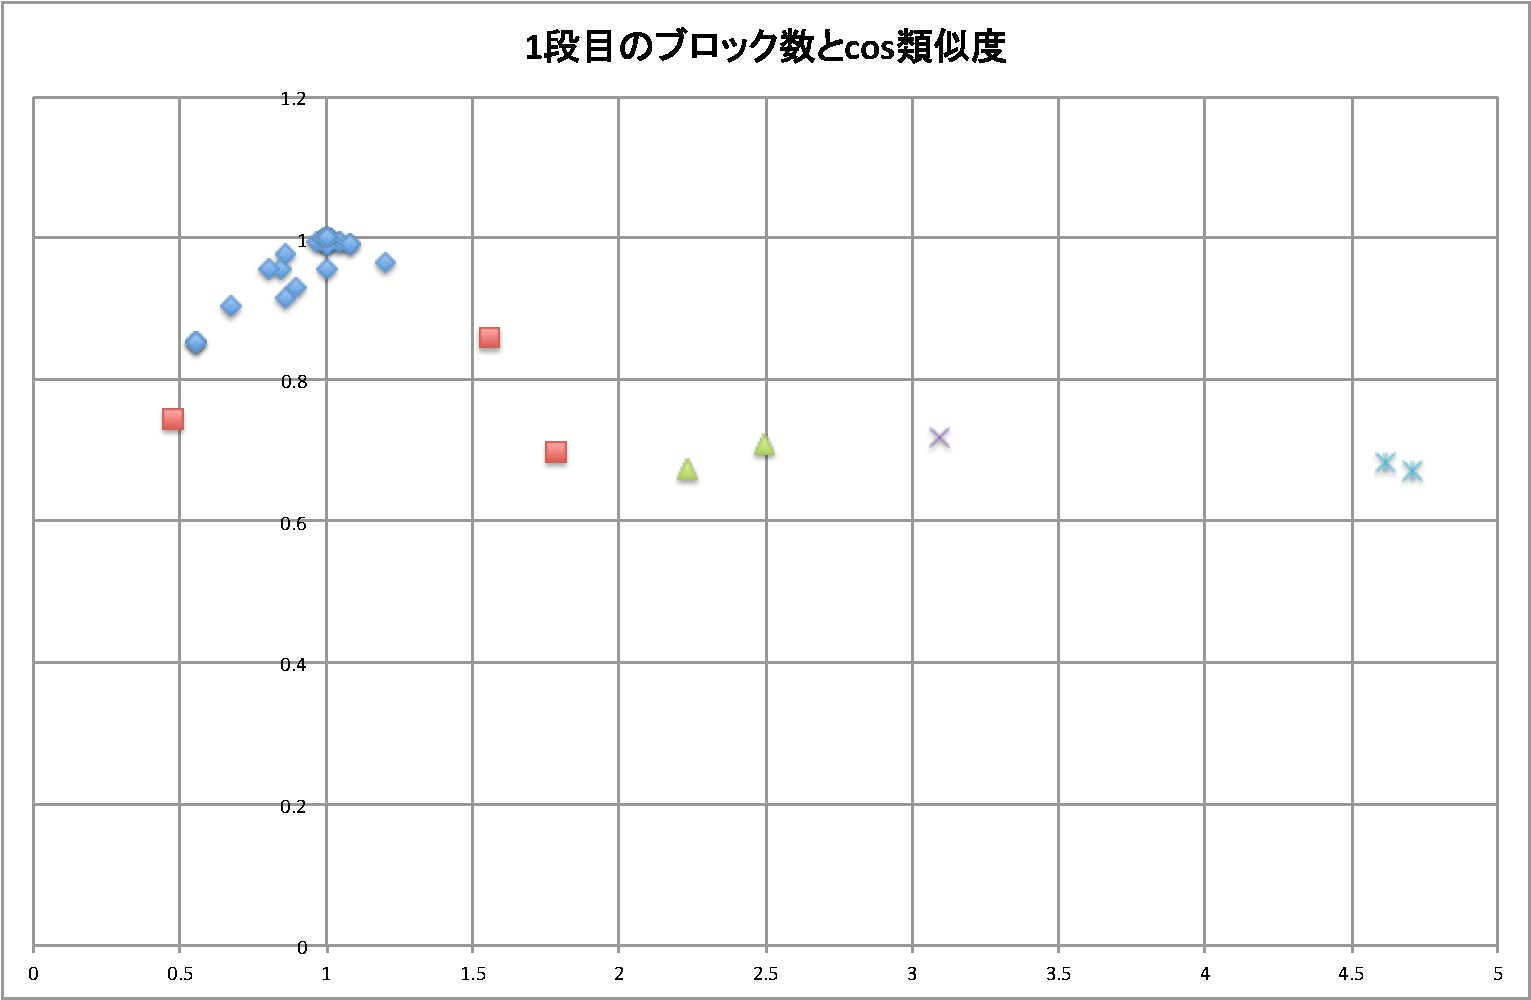
\includegraphics[keepaspectratio, scale = 0.14]{mazegame_first_block.pdf}
	 \caption{1段目のグラフ}
	 \label{first_block}
	\end{minipage}
        \begin{minipage}[t]{0.45\hsize}
	 \centering
	 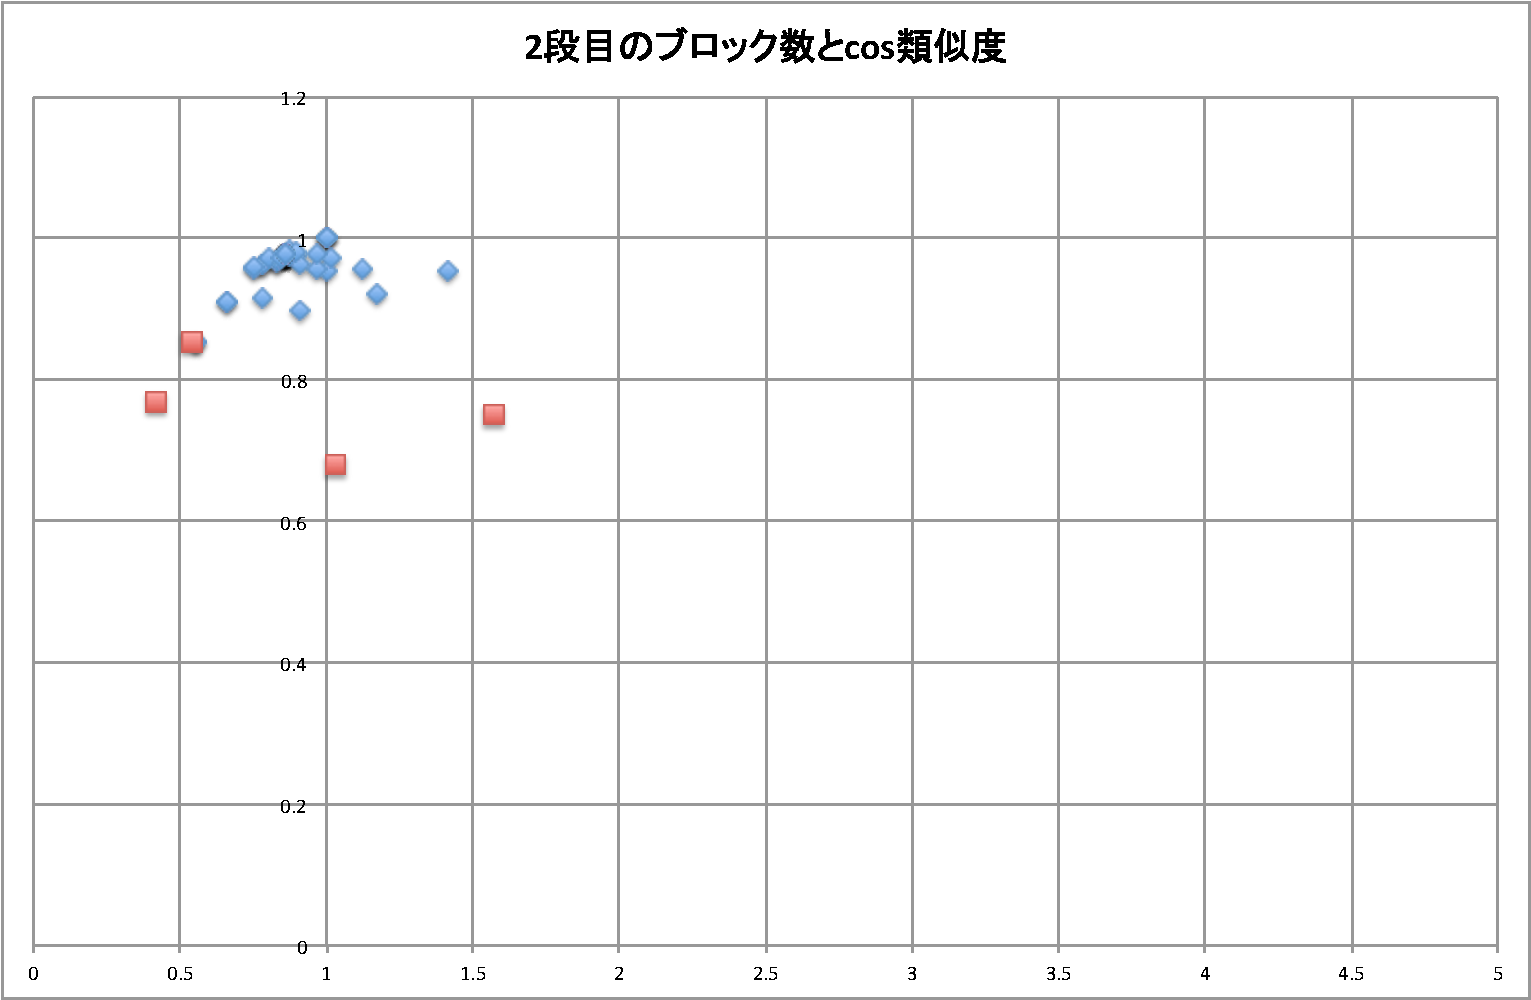
\includegraphics[keepaspectratio, scale = 0.14]{mazegame_second_block.pdf}
	 \caption{2段目のグラフ}
	 \label{second_block}
	\end{minipage}
 \end{tabular}
 \end{figure}

\subsubsection{スプライト数とcos類似度の散布図}
\begin{figure}[ht]
 \begin{tabular}{cc}
 	\begin{minipage}[t]{0.45\hsize}
	 \centering
	 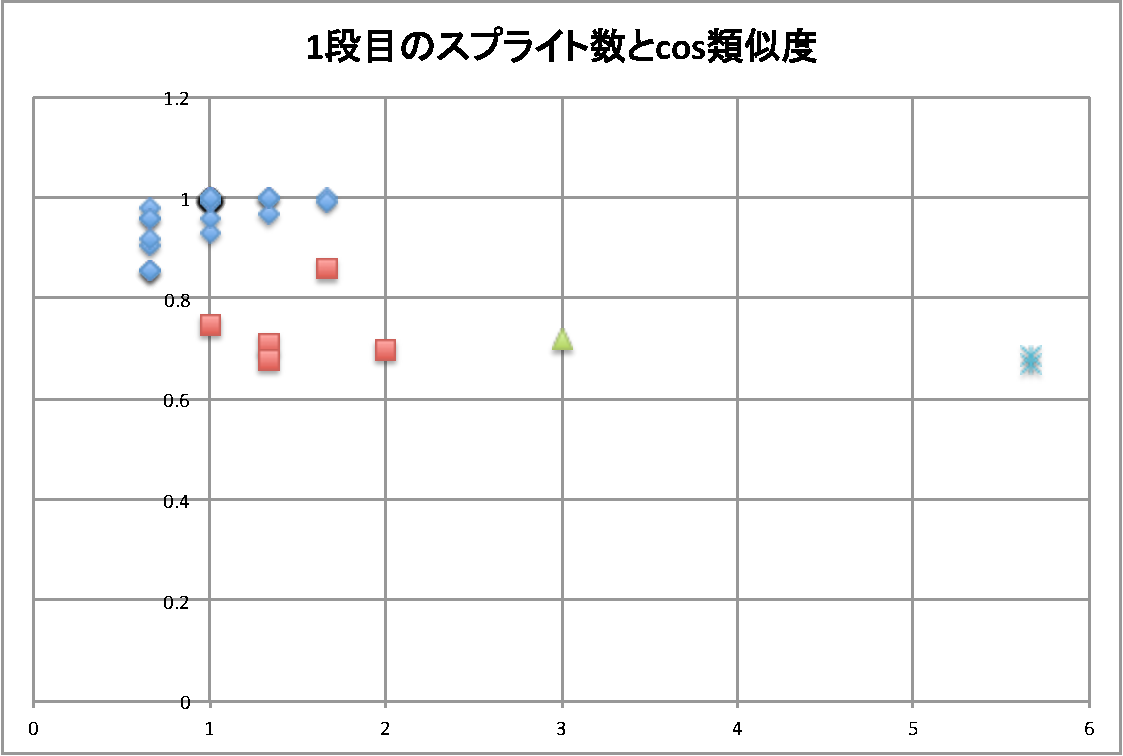
\includegraphics[keepaspectratio, scale = 0.14]{mazegame_first_splite.pdf}
	 \caption{1段目のグラフ}
	 \label{first_splite}
	\end{minipage}
        \begin{minipage}[t]{0.45\hsize}
	 \centering
	 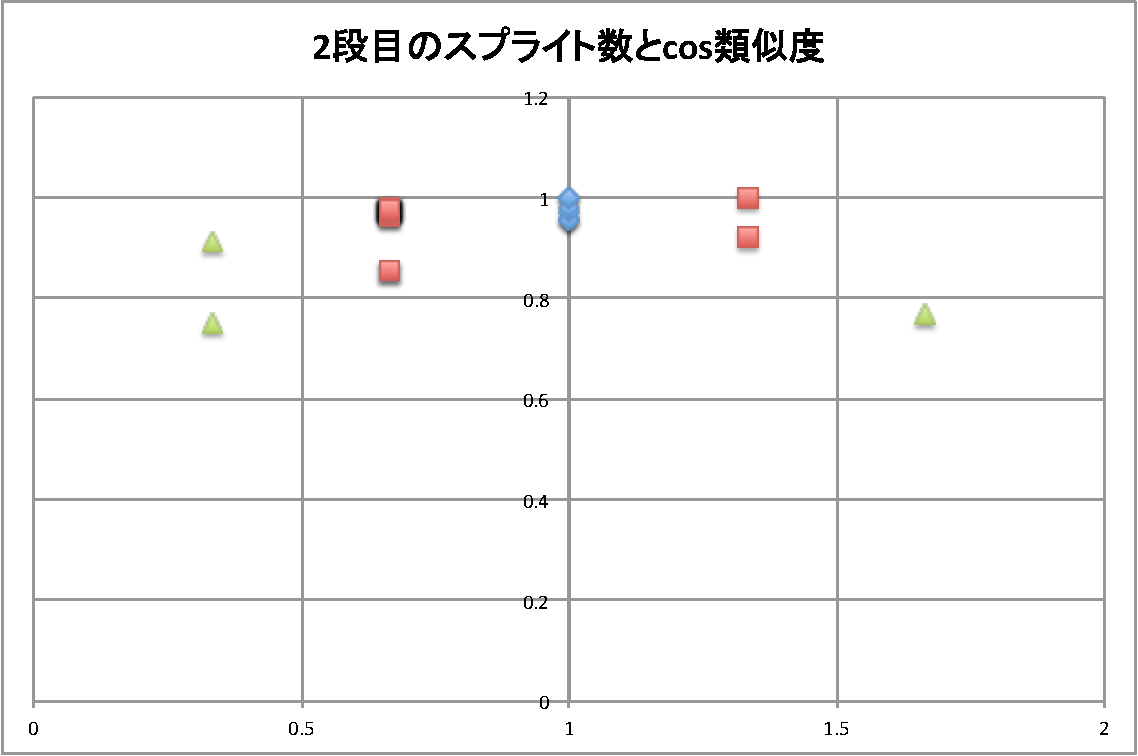
\includegraphics[keepaspectratio, scale = 0.14]{mazegame_second_splite.pdf}
	 \caption{2段目のグラフ}
	 \label{second_splite}
	\end{minipage}
 \end{tabular}
 \end{figure}


\section{評価}
作成したグラフ上の点をいくつかピックアップし、その点にあるプロジェクトを実際に動かして元プロジェクトとの類似度を操作・音・外装・プログラムの動き・ブロックの木構造・ゲーム終了時の6つの項目で比較してみたところ、それぞれの段で最も似ているもの・最も離れているもの・中間という条件で取り出したプロジェクトは、やはりよく似ている・違う・少し違う内容となっていた。情報科の学生にとったアンケートでも可視化して見えてきた類似度の位置関係と、実際に動かすことで分かる類似度は、ほぼ同じであることが分かった。よって、今回使用したブロック数・スプライト数・類似度はプロジェクト同士の類似度を図る上で重要な要素であったと言える。
\\
 また、1段目から4段目まですべてを通して見てみると、2段目以降にも元プロジェクトと同じような内容のものが含まれていることが分かった。これは、リミックスツリーの根元(元プロジェクト)から離れたプロジェクトも、元プロジェクトと同じ場合が生じているということが言え、リミックスツリーではその事実までは可視化されていなかったということが伺える。本研究で行った可視化手法では、例え元プロジェクトへいくつも遡るところに位置するプロジェクトであったとしても、ほぼ正確な類似関係が可視化できており、新たな可視化として提案できるのではないか。ここに本研究の新奇性を見出すことができた。
\\
 この可視化がツール上に加わることで、それぞれの生徒がどの程度自分のアイデアでプロジェクトを作成できているか、もしくはできていないのかという新たな情報を提供でき、教育者にとって個々の生徒の進度を把握する一つの手助けになるのではないかと考えている。

\section{今後の課題}


\begin{thebibliography}{6}
\bibitem{preEssay1}森秀樹・杉澤学・張海・前迫孝憲(2011)「Scratchを用いた小学校プログラミング授業の実践〜小学生を対象としたプログラミング教育の再考〜」
\bibitem{preEssay2}小田悠介、若林茂(2013) 「プログラム間の類似性の定量化手法」,[online]http://www.kobe-kosen.ac.jp/activity/publication/kiyou/Kiyou12/Data/Vol51Paper103-108.pdf
\bibitem{json_py}【Python入門】JSON形式データの扱い方 (2016年12月12日), Morio http://qiita.com/Morio/items/7538a939cc441367070d
\bibitem{cos} コサイン類似度 http://www.cse.kyoto-su.ac.jp/~g0846020/keywords/cosinSimilarity.html
\bibitem{pongret}Remix tree for Pong Starter https://scratch.mit.edu/projects/10000036/remixtree/
\bibitem{mazeret}Remix tree for Maze Game https://scratch.mit.edu/projects/2768574/remixtree/

\end{thebibliography}

%
%
\end{document}
